\documentclass[11pt]{article}
\usepackage[margin=2cm]{geometry}

% Core packages
\usepackage{amsmath,amssymb}
\usepackage{tikz-cd}
\usepackage{tikz}
\usepackage{multicol}
\renewcommand{\contentsname}{Índice}
\setcounter{tocdepth}{3}

% Paragraphs
\setlength{\parindent}{0pt}
\setlength{\parskip}{1\baselineskip}

\title{Notas de clase de Astroestadística}
\author{Daniel Soto Villada}
\date{Semestre 2026\text{-}2\\\today}

\begin{document}
\maketitle
\begingroup
\setlength{\parskip}{0pt}
\tableofcontents
\endgroup

\section{Clase 1}
\subsection{Generación de variables aleatorias por transformación inversa}

\subsubsection{De una densidad a una función de distribución}

Muchos métodos de simulación parten de un generador de números uniformes
independientes, $U\sim\mathcal{U}(0,1)$. La transformación inversa convierte
esos valores uniformes en observaciones con una distribución objetivo.

Una función $f$ es una densidad de probabilidad si $f(x)\geq0$ y su integral
sobre todo el soporte vale uno. La función de distribución acumulada (FDA) es
\[
    F(x)=\Pr(X\leq x)=\int_{-\infty}^{x} f(t)\,dt.
\]
La FDA es no decreciente y toma valores entre cero y uno. Si se parte de una
función no negativa $\tilde f$ que no está normalizada, primero se calcula
$c=\int_{-\infty}^{\infty}\tilde f(t)\,dt$ y se usa la densidad
$f(x)=\tilde f(x)/c$.

Cuando $F$ es continua y estrictamente creciente, tiene inversa. En ese caso,
la regla de generación es
\[
    U\sim\mathcal{U}(0,1),\qquad X=F^{-1}(U).
\]
En efecto, para cualquier $x$,
\[
    \Pr(X\leq x)
    =\Pr\bigl(F^{-1}(U)\leq x\bigr)
    =\Pr\bigl(U\leq F(x)\bigr)
    =F(x),
\]
por lo que $X$ tiene precisamente la distribución deseada. Si $F$ no es
estrictamente creciente, se utiliza la inversa generalizada
\[
    F^{-1}(u)=\inf\{x\in\mathbb{R}:F(x)\geq u\}.
\]
Esta definición también sirve para distribuciones discretas.

\subsubsection{Algoritmo}

Para generar $N$ observaciones independientes:
\begin{enumerate}
    \item Obtener $N$ valores independientes $U_1,\ldots,U_N$ de una uniforme
    en $(0,1)$.
    \item Calcular $X_i=F^{-1}(U_i)$ para cada $i=1,\ldots,N$.
    \item Usar $X_1,\ldots,X_N$ como la muestra de la distribución objetivo.
\end{enumerate}
El paso esencial es encontrar o evaluar la inversa de la FDA\@. A continuación
se muestran ejemplos donde esa operación puede hacerse explícitamente.

\subsubsection{Ejemplo 1: una densidad creciente en $[0,1]$}

Sea
\[
    f(x)=\begin{cases}2x,&0\leq x\leq1,\\0,&\text{en otro caso.}\end{cases}
\]
La integral de $f$ entre cero y uno es uno. En el intervalo de interés, su FDA
y su inversa son
\[
    F(x)=\int_0^x 2t\,dt=x^2,
    \qquad F^{-1}(u)=\sqrt{u}.
\]
Por tanto, basta generar $U\sim\mathcal{U}(0,1)$ y tomar $X=\sqrt U$. Por
ejemplo, si $U=0.36$, entonces $X=0.6$. La transformación favorece valores
cercanos a uno, como corresponde a una densidad $f(x)$ que crece en ese
sentido. La figura compara la densidad con la FDA, que acumula el área bajo
ella.

\begin{figure}[htbp]
\centering
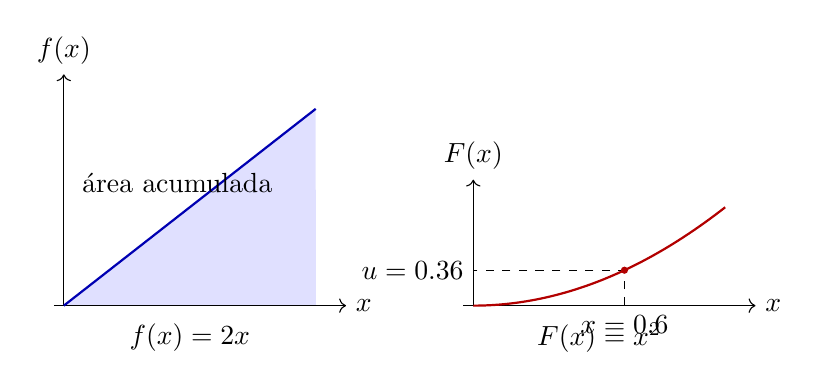
\begin{tikzpicture}[x=3.2cm,y=1.25cm]
  \begin{scope}
    \fill[blue!12] (0,0) -- plot[domain=0:1,samples=50] (\x,{2*\x}) -- (1,0) -- cycle;
    \draw[->] (-0.04,0) -- (1.12,0) node[right] {$x$};
    \draw[->] (0,0) -- (0,2.35) node[above] {$f(x)$};
    \draw[thick,blue!70!black,domain=0:1,samples=50] plot (\x,{2*\x});
    \node[below] at (0.5,-0.08) {$f(x)=2x$};
    \node at (0.45,1.25) {área acumulada};
  \end{scope}
  \begin{scope}[xshift=5.2cm]
    \draw[->] (-0.04,0) -- (1.12,0) node[right] {$x$};
    \draw[->] (0,0) -- (0,1.28) node[above] {$F(x)$};
    \draw[thick,red!70!black,domain=0:1,samples=50] plot (\x,{\x*\x});
    \draw[dashed] (0.6,0) -- (0.6,0.36) -- (0,0.36);
    \fill[red!70!black] (0.6,0.36) circle (1.3pt);
    \node[below] at (0.5,-0.08) {$F(x)=x^2$};
    \node[left] at (0,0.36) {$u=0.36$};
    \node[below] at (0.6,0) {$x=0.6$};
  \end{scope}
\end{tikzpicture}
\caption{La FDA $F(x)=x^2$ integra la densidad $f(x)=2x$. El nivel $u=0.36$ corresponde al cuantil $x=F^{-1}(u)=0.6$.}\label{fig:clase1-densidad-fda}
\end{figure}

\subsubsection{Ejemplo 2: distribución exponencial}

La distribución exponencial de tasa $\lambda>0$ tiene densidad
\[
    f(x)=\begin{cases}\lambda e^{-\lambda x},&x\geq0,\\0,&x<0.\end{cases}
\]
Al integrar se obtiene $F(x)=1-e^{-\lambda x}$ para $x\geq0$. Despejando $x$
en $u=F(x)$,
\[
    u=1-e^{-\lambda x}
    \quad\Longrightarrow\quad
    F^{-1}(u)=-\frac{1}{\lambda}\ln(1-u).
\]
Así, si $U\sim\mathcal{U}(0,1)$, la variable
\[
    X=-\frac{1}{\lambda}\ln(1-U)
\]
sigue la distribución exponencial de tasa $\lambda$. Como $1-U$ también es
uniforme en $(0,1)$, se usa a menudo la forma equivalente
$X=-\ln(U)/\lambda$. Por ejemplo, con $\lambda=1$ y $U=0.7$,
$X=-\ln(0.3)\approx1.204$.

En la primera figura se ve cómo una altura uniforme $u$ selecciona un punto
sobre la función de distribución acumulada. La segunda muestra la misma
operación usando la curva inversa.

\begin{figure}[htbp]
\centering
\begin{tikzpicture}[x=2.1cm,y=3.0cm]
  \draw[->] (-0.08,0) -- (3.35,0) node[right] {$x$};
  \draw[->] (0,0) -- (0,1.12) node[above] {$F(x)$};
  \draw[thick,blue!70!black,domain=0:3,samples=80] plot (\x,{1-exp(-\x)});
  \draw[dashed] (0,0.7) -- (1.204,0.7) -- (1.204,0);
  \fill[blue!70!black] (1.204,0.7) circle (1.5pt);
  \node[left] at (0,0.7) {$U=0.7$};
  \node[below] at (1.204,0) {$X=-\ln(0.3)\approx1.204$};
  \node[blue!70!black,anchor=west] at (2.1,0.82) {$F(x)=1-e^{-x}$};
\end{tikzpicture}
\caption{Para una exponencial de tasa $\lambda=1$, el valor uniforme $U=0.7$ se traza hasta la FDA y determina el cuantil $X=F^{-1}(0.7)$.}\label{fig:clase1-mapeo-fda}
\end{figure}
\begin{figure}[htbp]
\centering
\begin{tikzpicture}[x=6cm,y=1.8cm]
  \draw[->] (-0.03,0) -- (1.04,0) node[right] {$u$};
  \draw[->] (0,0) -- (0,3.45) node[above] {$F^{-1}(u)$};
  \draw[thick,red!70!black,domain=0.01:0.96,samples=90] plot (\x,{-ln(1-\x)});
  \draw[dashed] (0.7,0) -- (0.7,1.204) -- (0,1.204);
  \fill[red!70!black] (0.7,1.204) circle (1.5pt);
  \node[below] at (0.7,0) {$0.7$};
  \node[left] at (0,1.204) {$1.204$};
  \node[anchor=west] at (0.12,3.1) {$F^{-1}(u)=-\ln(1-u)$};
\end{tikzpicture}
\caption{La FDA inversa transforma cualquier $U$ uniforme en un valor exponencial. Aquí se muestra de nuevo $U=0.7$.}\label{fig:clase1-inversa}
\end{figure}

\subsubsection{Distribuciones discretas e inversas no explícitas}

Para una variable discreta con valores $x_1<x_2<\cdots<x_k$ y probabilidades
$p_1,\ldots,p_k$, se acumulan las probabilidades y se devuelve el primer $x_j$
cuya suma acumulada es al menos $U$. Por ejemplo, si
\[
    \Pr(X=0)=0.2,\qquad \Pr(X=1)=0.5,\qquad \Pr(X=2)=0.3,
\]
la regla es
\[
    X=\begin{cases}
        0,&0<U\leq0.2,\\
        1,&0.2<U\leq0.7,\\
        2,&0.7<U<1.
    \end{cases}
\]
La longitud de cada intervalo es igual a la probabilidad del valor que le
corresponde.

No siempre se puede despejar $F^{-1}$ mediante una fórmula elemental. Si se
puede evaluar $F(x)$, se puede hallar $x$ resolviendo $F(x)=U$ numéricamente;
por ejemplo, mediante búsqueda por bisección cuando $F$ es monótona. La
transformación inversa es especialmente sencilla cuando la FDA y su inversa
son fáciles de calcular.

\subsubsection{Resumen}

La transformación inversa convierte una muestra uniforme en una muestra con
la FDA deseada: se calcula $F$ integrando la densidad normalizada, se genera
$U\sim\mathcal{U}(0,1)$ y se obtiene $X=F^{-1}(U)$. Para una FDA discreta o no
estrictamente creciente se usa la inversa generalizada.
\section{Clase 2}
\subsection{Muestreo por aceptación y rechazo}

\subsubsection{La idea geométrica}

El método de aceptación y rechazo permite generar observaciones de una
distribución objetivo cuando es más fácil generar observaciones de otra
distribución. La idea es proponer valores con una distribución conocida y
conservar cada propuesta con una probabilidad que favorezca las regiones donde
la distribución objetivo tiene mayor densidad.

Hay una distinción importante en la notación. Denotemos por $f(x)$ la densidad
objetivo y por $q(x)$ la densidad de propuesta, ambas normalizadas. Se busca una
constante $M\geq 1$ tal que
\[
    f(x)\leq Mq(x)\qquad\text{para todo }x.
\]
La función $h(x)=Mq(x)$ es la envolvente, y el cociente
\[
    \frac{f(x)}{h(x)}=\frac{f(x)}{Mq(x)}
\]
es una probabilidad válida de aceptación. En particular, se genera $x$ según
$q$ (no según la envolvente sin normalizar) y se acepta si
$U\leq f(x)/(Mq(x))$, donde $U\sim\mathcal{U}(0,1)$. Si se llama $g$ a la
propuesta, la envolvente correspondiente es $Mg$; de ese modo se evita
confundir una densidad normalizada con una cota que puede tener área mayor que
uno.

\subsubsection{Ejemplo: generar observaciones con densidad $f(x)=2x$}

Consideremos la densidad objetivo
\[
    f(x)=2x,\quad 0\leq x\leq 1,
    \qquad f(x)=0\text{ fuera de }[0,1].
\]
Su integral en $[0,1]$ es uno. Elegimos como propuesta la uniforme
$q(x)=1$ en ese intervalo. Como $f(x)\leq 2q(x)$, podemos tomar $M=2$; la
envolvente es $h(x)=Mq(x)=2$. Para cada propuesta $x\sim\mathcal{U}(0,1)$, la
regla se reduce a
\[
    \text{aceptar }x\quad\Longleftrightarrow\quad
    U\leq\frac{f(x)}{Mq(x)}=x,
    \qquad U\sim\mathcal{U}(0,1).
\]
Por ejemplo, si la propuesta es $x=0.7$, se acepta cuando $U\leq0.7$; si es
$x=0.2$, se acepta cuando $U\leq0.2$. Las propuestas cercanas a uno tienen
mayor probabilidad de sobrevivir, tal como requiere la forma creciente de
$f$.

Una corrida ilustrativa puede dar estos resultados: para $(x,U)=(0.16,0.18)$
se rechaza, pues $0.18>0.16$; para $(0.32,0.11)$ se acepta, pues
$0.11\leq0.32$; para $(0.70,0.55)$ se acepta, y para $(0.86,0.90)$ se
rechaza. En cada intento se genera una propuesta nueva; los valores aceptados
se guardan hasta reunir la cantidad deseada.
\begin{figure}[htbp]
\centering
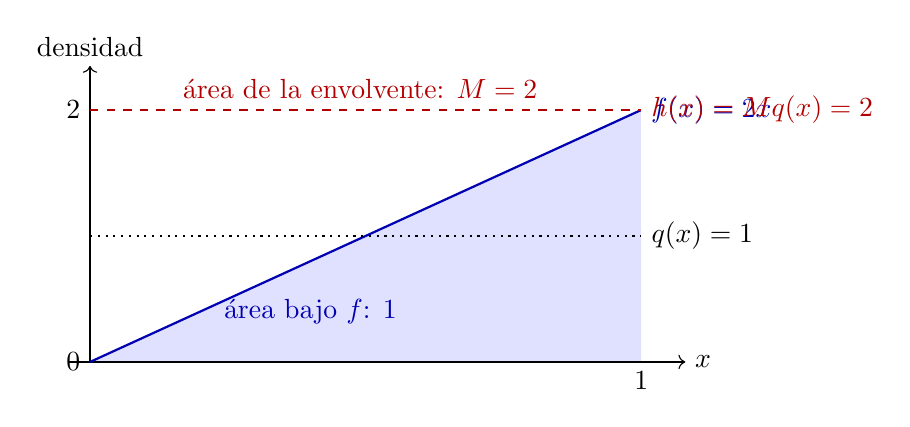
\begin{tikzpicture}[x=7cm,y=1.6cm]
  \fill[blue!12] (0,0) -- plot[domain=0:1,samples=60] (\x,{2*\x}) -- (1,0) -- cycle;
  \draw[->] (-0.04,0) -- (1.08,0) node[right] {$x$};
  \draw[->] (0,0) -- (0,2.35) node[above] {densidad};
  \draw[thick,blue!70!black,domain=0:1,samples=60] plot (\x,{2*\x})
    node[right] {$f(x)=2x$};
  \draw[thick,dashed,red!70!black] (0,2) -- (1,2)
    node[right] {$h(x)=Mq(x)=2$};
  \draw[thick,dotted] (0,1) -- (1,1)
    node[right] {$q(x)=1$};
  \draw (0,0) node[left] {$0$};
  \draw (0,2) node[left] {$2$};
  \draw (1,0) node[below] {$1$};
  \node[blue!70!black] at (0.40,0.40) {área bajo $f$: $1$};
  \node[red!70!black] at (0.49,2.17) {área de la envolvente: $M=2$};
\end{tikzpicture}
\caption{La densidad objetivo queda debajo de la envolvente. La propuesta es uniforme en $[0,1]$.}\label{fig:envolvente}
\end{figure}

\subsubsection{Procedimiento paso a paso}

Para obtener $N$ observaciones aceptadas:
\begin{enumerate}
    \item Especificar la densidad objetivo $f$ y una propuesta $q$ fácil de
    simular.
    \item Encontrar $M$ tal que $f(x)\leq Mq(x)$ en todo el soporte.
    \item Generar una propuesta $x\sim q$.
    \item Generar $U\sim\mathcal{U}(0,1)$, independiente de $x$.
    \item Aceptar y guardar $x$ si $U\leq f(x)/(Mq(x))$; en caso contrario,
    descartarlo.
    \item Repetir desde el paso 3 hasta reunir $N$ valores aceptados.
\end{enumerate}

En el ejemplo, el paso de aceptación es $U\leq x$. Si se realizan $n$
propuestas, se espera aceptar aproximadamente $n/M=n/2$; por tanto, para
reunir $N$ valores aceptados se necesitan, en promedio, cerca de $2N$
propuestas. Algunas propuestas se descartan, pero los valores que se guardan
siguen la densidad $f$.

\begin{figure}[htbp]
\centering
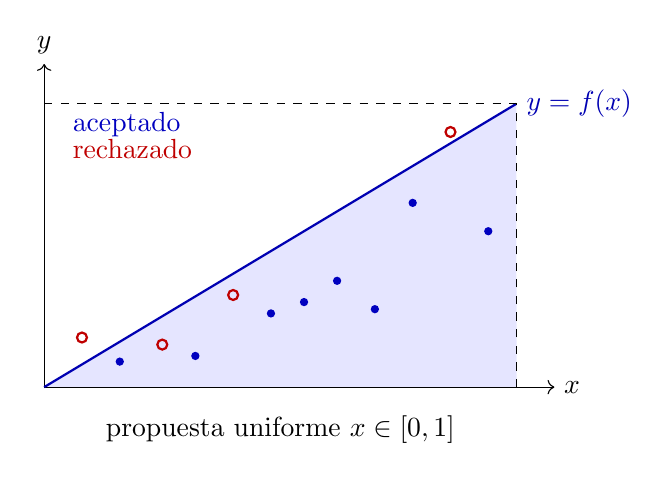
\begin{tikzpicture}[x=6cm,y=1.8cm]
  \fill[blue!10] (0,0) -- plot[domain=0:1,samples=60] (\x,{2*\x}) -- (1,0) -- cycle;
  \draw[->] (0,0) -- (1.08,0) node[right] {$x$};
  \draw[->] (0,0) -- (0,2.28) node[above] {$y$};
  \draw[thick,blue!70!black,domain=0:1,samples=60] plot (\x,{2*\x})
    node[right] {$y=f(x)$};
  \draw[dashed] (1,0) -- (1,2);
  \draw[dashed] (0,2) -- (1,2);
  \foreach \x/\y in {0.16/0.18,0.32/0.22,0.48/0.52,0.55/0.60,
                      0.62/0.75,0.70/0.55,0.78/1.30,0.94/1.10}
    \fill[blue!75!black] (\x,\y) circle (1.5pt);
  \foreach \x/\y in {0.08/0.35,0.25/0.30,0.40/0.65,0.86/1.80}
    \draw[red!75!black,thick] (\x,\y) circle (1.8pt);
  \node[blue!75!black,anchor=west] at (0.04,1.85) {aceptado};
  \node[red!75!black,anchor=west] at (0.04,1.68) {rechazado};
  \node[below] at (0.5,-0.13) {propuesta uniforme $x\in[0,1]$};
\end{tikzpicture}
\caption{Cada punto se propone uniformemente en el rectángulo $[0,1]\times[0,2]$. Se conserva si queda bajo $f(x)=2x$. Los puntos son ilustrativos.}\label{fig:puntos}
\end{figure}

\subsubsection{La relación con estimar áreas}

La misma regla se puede leer geométricamente: las propuestas uniformes caen
en un rectángulo de área $|R|$, y se aceptan las que caen bajo la curva. Si la
región bajo una función no negativa tiene área $A$, entonces, al generar $n$
puntos uniformes en el rectángulo y contar $N_0$ puntos aceptados,
\[
    \frac{N_0}{n}\approx\frac{A}{|R|},
    \qquad\text{así que}\qquad
    A\approx |R|\frac{N_0}{n}.
\]
Cuando el rectángulo tiene área uno, esto se simplifica a
$A\approx N_0/n$. En el ejemplo, el rectángulo envolvente tiene área $2$ y la
región bajo $f$ tiene área $1$, de modo que la fracción aceptada se aproxima a
$1/2$. Cuantas más propuestas se generen, más estable tiende a ser esta
estimación.

\begin{figure}[htbp]
\centering
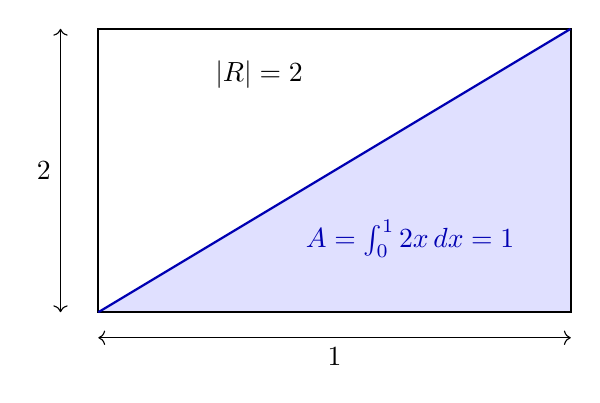
\begin{tikzpicture}[x=6cm,y=1.8cm]
  \fill[blue!12] (0,0) -- plot[domain=0:1,samples=60] (\x,{2*\x}) -- (1,0) -- cycle;
  \draw[thick] (0,0) rectangle (1,2);
  \draw[thick,blue!70!black,domain=0:1,samples=60] plot (\x,{2*\x});
  \draw[<->] (0,-0.18) -- (1,-0.18) node[midway,below] {$1$};
  \draw[<->] (-0.08,0) -- (-0.08,2) node[midway,left] {$2$};
  \node[blue!70!black] at (0.66,0.52) {$A=\int_0^1 2x\,dx=1$};
  \node at (0.34,1.68) {$|R|=2$};
\end{tikzpicture}
\caption{El cociente entre el área sombreada y el área del rectángulo es la probabilidad de aceptación.}\label{fig:area}
\end{figure}

\subsubsection{¿Por qué funciona?}

Una propuesta $x$ tiene densidad $q(x)$ y se acepta con probabilidad
$f(x)/(Mq(x))$. Por lo tanto, la densidad conjunta de propuestas aceptadas
es proporcional a
\[
    q(x)\frac{f(x)}{Mq(x)}=\frac{f(x)}{M}.
\]
Al normalizar esta expresión se obtiene precisamente $f(x)$. La probabilidad
de aceptación total es $1/M$ cuando $f$ y $q$ son densidades normalizadas.
Conviene elegir una envolvente ajustada: si $M$ es innecesariamente grande,
se rechazan más propuestas y el algoritmo se vuelve menos eficiente.

\end{document}
